%% LaTeX Beamer presentation template (requires beamer package)
%% see http://bitbucket.org/rivanvx/beamer/wiki/Home
%% idea contributed by H. Turgut Uyar
%% template based on a template by Till Tantau
%% this template is still evolving - it might differ in future releases!

\documentclass{beamer}

\mode<presentation>
{
\usetheme{Warsaw}

\setbeamercovered{transparent}
}

\usepackage[polish]{babel}
\usepackage[utf8]{inputenc}

% font definitions, try \usepackage{ae} instead of the following
% three lines if you don't like this look
\usepackage{mathptmx}
\usepackage[scaled=.90]{helvet}
\usepackage{courier}
\usepackage{graphicx}
\usepackage[square]{natbib}


\usepackage[T1]{fontenc}


\title{Peer-to-peer web objects caching proxy}

%s\subtitle{Chaum, Crepeau, Damgard}

% - Use the \inst{?} command only if the authors have different
%   affiliation.
%\author{F.~Author\inst{1} \and S.~Another\inst{2}}
\author{Tomasz Drwięga}

% - Use the \inst command only if there are several affiliations.
% - Keep it simple, no one is interested in your street address.
% \institute[Universities of]
% {
% \inst{1}%
% Department of Computer Science\\
% Univ of S
% \and
% \inst{2}%
% Department of Theoretical Philosophy\\
% Univ of E}

\date{08.05.2013 / Seminarium}


% This is only inserted into the PDF information catalog. Can be left
% out.
\subject{Talks}



% If you have a file called "university-logo-filename.xxx", where xxx
% is a graphic format that can be processed by latex or pdflatex,
% resp., then you can add a logo as follows:

% \pgfdeclareimage[height=0.5cm]{university-logo}{university-logo-filename}
% \logo{\pgfuseimage{university-logo}}


% If you wish to uncover everything in a step-wise fashion, uncomment
% the following command:

%\beamerdefaultoverlayspecification{<+->}

\begin{document}

\begin{frame}
\titlepage
\end{frame}

\begin{frame}
\frametitle{Agenda}
\tableofcontents
% You might wish to add the option [pausesections]
\end{frame}


% \section{Sformułowanie problemu}

\begin{frame}
\frametitle{Sformułowanie problemu}
Problem cache'owania można przedstawić z różnych perspektyw.

\begin{block}{Dostawca treści}
Wiele żądań może spowodować ``zalanie'' (ang. \textit{flooding, swamping}) serwera.
\end{block}
\begin{block}{Administrator sieci}
Wielokrotny transfer tego samego zasobu może prowadzić do obniżenia jakości usług.
\end{block}
\begin{block}{Użytkownicy}
Pobieranie dużych plików z odległych serwerów może odbywać się ze znaczącym opóźnieniem.
\end{block}
\end{frame}


\section{Poprzednie prace}
\subsection{Harvest (Squid) object cache}

\begin{frame}
\frametitle{Squid object cache}
\centering
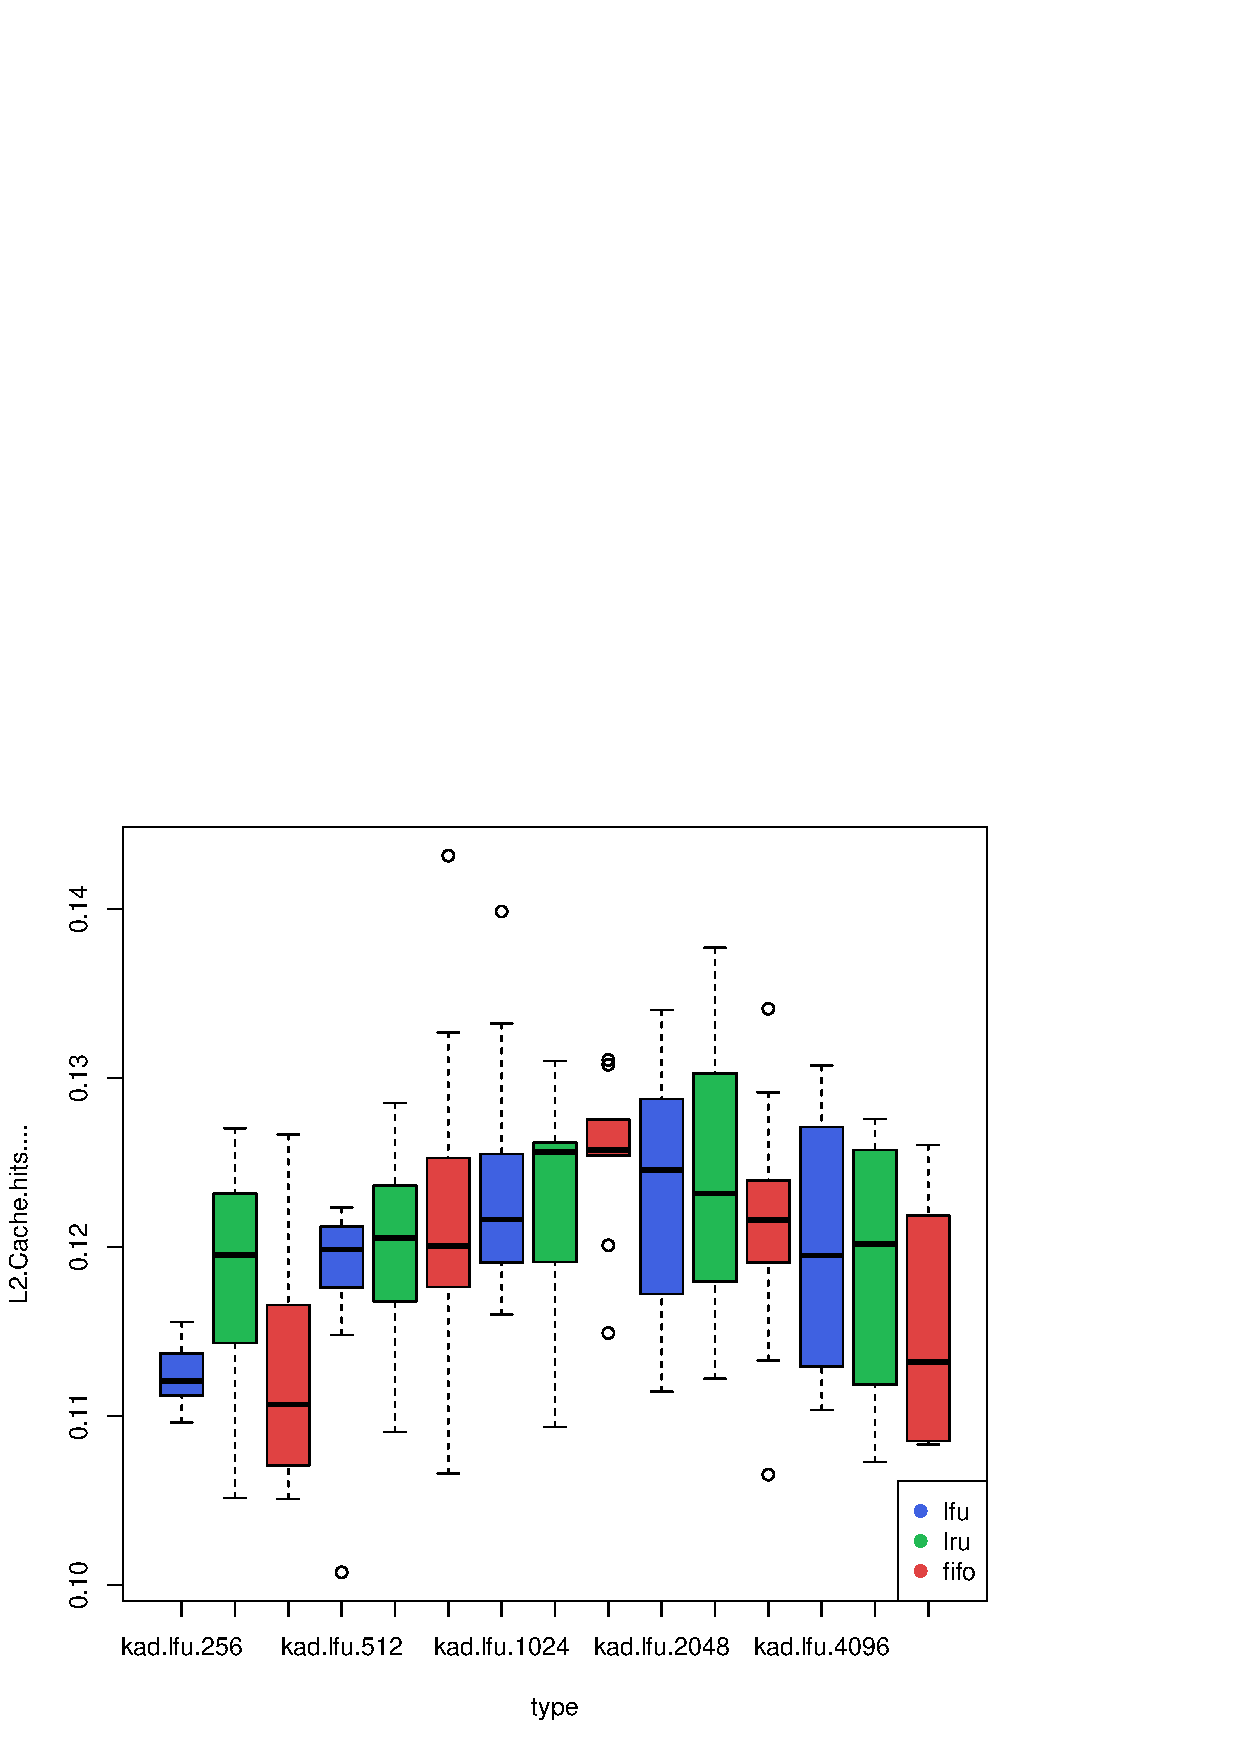
\includegraphics[width=0.8\linewidth]{img/cache.pdf}

\begin{block}{}
Rozwiązanie: Wprowadzenie serwerów pośredniczących, które będą powielać oryginalne zasoby.
\end{block}

\end{frame}


\begin{frame}
\frametitle{Cache hierarchiczny}
\begin{block}{}
Wiele serwerów cache'ujących można zorganizować w hierarchię \citep{chankhunthod1995hierarchical}.
\end{block}

\begin{columns}[c]
\column{0.45\textwidth}
\begin{center}
\includegraphics[width=0.8\linewidth]{img/hierarchical.pdf}
\end{center}

\column{0.5\textwidth}
\pause
\begin{block}{}
Serwery, znajdujące się w liściach mogą wymieniać się zasobami (cache kooperacyjny). Prowadzi to jednak do nadmiernej komunikacji \citep{povey1997distributed, wolman1999scale}.
\end{block}

\end{columns}

\end{frame}

\subsection{Consistent Hashing}

\begin{frame}
\frametitle{W kierunku Consistent Hashing \citep{karger1997consistent}}
\begin{block}{}
Głównym problemem w systemach cache'ujących jest określenie, który z serwerów może być odpowiedzialny za dany zasób. 
\end{block}

\pause
\begin{block}{Naiwny podział}
Załóżmy, że poszukujemy zasobu $R$, który przydzielamy do serwera o indeksie $S$: 
\begin{equation*}
S \equiv hash(R) \bmod n
\end{equation*}
\end{block}

\pause
\begin{block}{}
Kiedy dodajemy lub usuwamy serwery, niemal każdy zasób przydzielony jest do innego serwera.
\end{block}

\end{frame}


\begin{frame}
\frametitle{Consistent hashing}

\begin{block}{}
Celem jest poprawienie procesu dodawania i usuwania węzłów tak, żeby nowy serwer przejął równy udział od pozostałych.
\end{block}

\begin{columns}[c]
\column{0.5\textwidth}

\begin{center}
\includegraphics[width=0.75\linewidth]{img/consistent.pdf}
\end{center}

\column{0.5\textwidth}
\begin{block}{Consistent hashing}
Każdy węzeł (oraz każdy zasób) jest mapowany do punktu na okręgu jednostkowym.
Węzeł jest odpowiedzialny za klucze, które znajdują się między nim a jego poprzednikiem \citep{karger1999web}. 
\end{block}

\end{columns}

\end{frame}



\subsection{DHT - Kademlia}

\begin{frame}
\frametitle{Rozproszone Tablice Haszujące (DHT)}

\begin{block}{}
Zdecentralizowany (autonomiczny), samo-organizujący się system typu peer-to-peer, oferujący usługę przypominającą tablicę haszującą.
DHT są dodatkowo odporne na błędy i skalowalne.
\end{block}

\pause
\begin{block}{}
Badania nad DHT były motywowane istniejącymi systemami:
\begin{description}
  \item[Napster] P2P z centralnym serwerem indeksującym
  \item[Gnutella] P2P rozsyłające zapytanie do każdego z węzłów w pewnym promieniu
  \item[Freenet] w pełni rozproszony, ale nie gwarantujący, że dane zostaną odnalezione
\end{description}
\end{block}

\begin{block}{Cztery główne DHT (2001)}
CAN, Chord, Pastry, Tapestry
\end{block}

\end{frame}

\begin{frame}
\frametitle{Kademlia \citep{maymounkov2002kademlia}}
\begin{block}{}
Podobnie jak pozostałe DHT, Kademlia podczas wyszukiwania kontaktuje się tylko z $O(\log n)$ węzłami.
\end{block}

\pause

\begin{block}{}
Każdemu węzłowi przypisany jest 160-bitowy klucz. Węzeł utrzymuje tablicę routingu, w której przechowuje listy (\textit{$k$-buckets}) węzłow, z którymi dzieli prefiks długości $i$, ale różni się na na bicie $i+1$.
Takie \textit{$k$-buckets} istnieją dla każdego $i \in [0, 160)$.
\end{block}

\begin{center}
\includegraphics[width=0.55\linewidth]{img/kademlia.pdf}
\end{center}

\end{frame}

\begin{frame}
\frametitle{Kademlia - metryka XOR}

\begin{block}{}
Kademlia korzysta z metryki XOR to określenia odległości między węzłami. Oznacza to, że węzły, które mają długi wspólny prefiks są blisko siebie. Upraszcza to formalną analizę, dowód poprawności i implementację.
\end{block}

\pause

\begin{block}{}
Wiadomości protokołu:
\begin{description}
\item[PING] weryfikuje, że węzeł jest aktywny,
\item[STORE] prosi węzeł o zapamiętanie pary (klucz, wartość)
\item[FIND\_NODE] zwraca $k$ najbliższych węzłów dla zadanego ID
\item[FIND\_VALUE] zwraca $k$ najbliższych węzłów lub przypisaną wartość dla danego ID
\end{description}
\end{block}

\end{frame}

% \begin{frame}
% \frametitle{Kademlia - porównanie}
% 
% \begin{block}{}
% Metryka XOR upraszcza algorytm routingu - w przeciwieństwie do Pastry czy Tapestry ten sam algorytm jest używany podczas całego procesu.
% \end{block}
% 
% \pause
% 
% \begin{block}{}
% Ponieważ XOR jest ???jednokierunkowa??? (czyli dla dowolnego $x$ i $\Delta$ istnieje tylko jeden $y$ taki, że $d(x, y) = \Delta$) wyszukiwania tego samego klucza zbiegają po tych samych ścieżkach.
% 
% Zatem możliwe jest cache'owanie par (klucz, wartośc) na węzłach znajdujących się na tej ścieżce.
%  
% \end{block}
% 
% \pause
% 
% \begin{block}{}
% Takie cache'owanie pozwala na przyspieszenie wyszukiwania popularnych zasobów w sieci.
% \end{block}
% 
% \end{frame}

\section{P2P Caching}
\begin{frame}
\frametitle{P2P Caching}

\begin{block}{}
Zamiast pobierać zasoby z oryginalnego serwera przeszukujemy najpierw rozproszoną tablicę haszującą, opartą na Kademli.
\end{block}

\begin{block}{Potencjalne zalety}
\begin{itemize}
  \item ``Duże'' zasoby mogą zostać pobrane szybciej (węzły należą do tej samej sieci LAN)
  \item Przepustowość łącza WAN jest oszczędzana
\end{itemize}
\end{block}

\end{frame}

\begin{frame}
\frametitle{P2P Caching - Implementacja}

\begin{block}{Pierwsza próba: Wtyczka przeglądarkowa w Javascript}
Łatwa w instalacji wtyczka używająca nowych API z HTML5.

\textbf{Dlaczego nie?} Żądania musiałyby być przetwarzane synchronicznie.
\end{block}

\pause
\begin{block}{Wtyczka Native Client dla Chrome}
Łatwa w instalacji, oferująca dobrą wydajność, ale ograniczona tylko do przeglądarek Chrome.

\textbf{Dlaczego nie?} Brak dokumentacji, niewystarczające API.
\end{block}

\pause
\begin{block}{Fallback: Proxy cache'ujące}
Serwer proxy napisany w jęzku Python z użyciem frameworku Twisted i biblioteki Entangled.

\textbf{Wada:} Wymagana jest dodatkowa konfiguracji przeglądarki.
\end{block}

\end{frame}

\section{Wyzwania}
\begin{frame}
\frametitle{Wyzwania}

\begin{block}{Logika cache'owania}
W jaki sposób zarządzać zasobami w cache'u o ograniczonym rozmiarze.
\end{block}

\begin{block}{Równoważenie obciążenia}
Żądania o zasoby z tej samej strony internetowej mogą być routowane do zupełnie
innych części sieci z powodu losowego wyboru kluczy.
\end{block}

\begin{block}{Wybór / porównanie różnych DHT}
Pomimo tej samej teoretycznej złożoności routingu, różne sieci P2P
mogą istotnie różnić się w zastosowaniu praktycznym.
\end{block}

\end{frame}

\subsection{Algorytmy cache'owania}
\begin{frame}
\frametitle{Logika cache'owania}
\begin{columns}[c]

\column{0.4\textwidth}
\begin{center}
\includegraphics[width=\linewidth]{img/architecture.pdf}
\end{center}

\column{0.6\textwidth}
\begin{block}{}
Pobieranie zasobu z sieci P2P zwiększa opóźnienie, 
popularne elementy warto przechowywać w pamięci.
\end{block}

\begin{block}{}
Porównanie różnych algorytmów:
\begin{itemize}
  \item LRU
  \item LFU
  \item FIFO
\end{itemize}
\end{block}

\end{columns}
\end{frame}

% \subsection{Równoważenie obciążenia}
% \begin{frame}
% \frametitle{Równoważenie obciążenia}
% 
% \begin{block}{}
% Wiele zasobów z jednej witryny, które pobierane są razem może zostać spakowane
% i umieszczone pod wspólnym kluczem w sieci P2P.
% \end{block}
% 
% \begin{block}{}
% Prosząc o pojedynczy zasób z sieci, otrzymujemy paczkę zawierającą zasoby, które
% prawdopodobnie będą nam potrzebne w najbliższej przyszłości.
% \end{block}
% 
% \end{frame}

\section{Przeprowadzone testy}
\begin{frame}
\frametitle{Wyniki eksperymentów}

\begin{block}{Dane testowe}
\begin{itemize}
  \item Problem ze znalezieniem aktualnych logów z serwerów (najnowsze z roku 2007).
  \item Możliwośc wygenerowania danych losowych 
\end{itemize}
\end{block}

\begin{block}{Porównanie z innymi rozwiązaniami}
\begin{itemize}
  \item Wyniki z prac bazują na przestarzałych danych
  \item Brak kodu lub warunków na uruchomienie aplikacji
\end{itemize}
\end{block}
\end{frame}

\begin{frame}
\frametitle{Wyniki eksperymentów}
\begin{block}{}
Użycie danych z serwera proxy z 2007 roku.
\end{block}

\begin{block}{Algorytmy}
Porównanie algorytmów cachowania: LRU, LFU i FIFO.
\end{block}
TOOD: !!!!
\begin{block}{Równoważenie obciążenia}
Grupowanie (bazowane na czasie) zasobów pochodzących z jednej strony (np. obrazki) pod wspólnym kluczem w sieci P2P.
\end{block}

\begin{block}{}
Porównanie opóźnień w Kademlii, Chordzie i Pastry.
\end{block}
TOOD: /!!!!

\end{frame}

\begin{frame}
\frametitle{Wyniki eksperymentów - Local Cache}
\begin{figure}
\centering
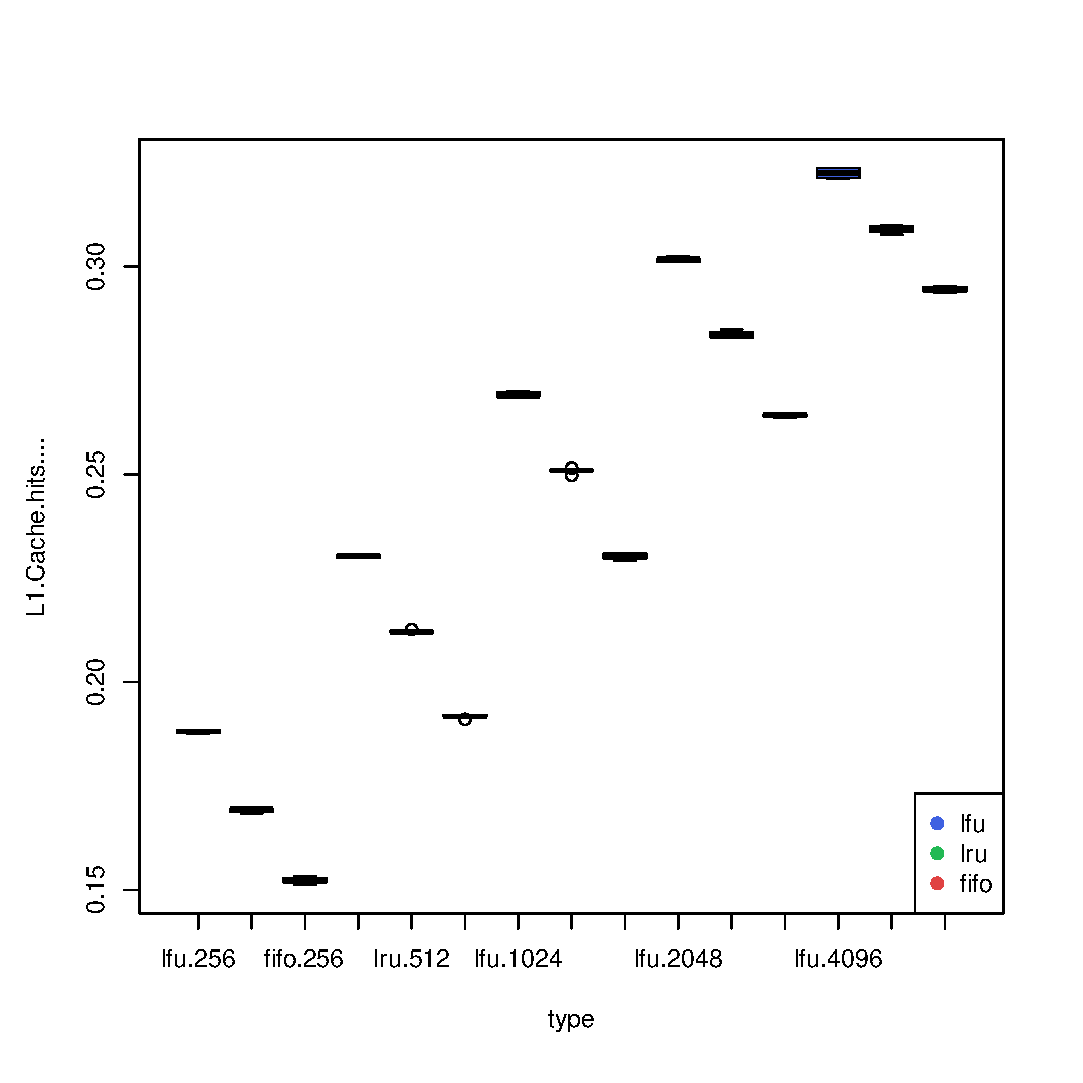
\includegraphics[width=0.7\linewidth]{img/tests/nop2p_all.eps}
\end{figure}
\end{frame}

\begin{frame}
\frametitle{Wyniki eksperymentów - P2P Cache}
\begin{figure}
\centering
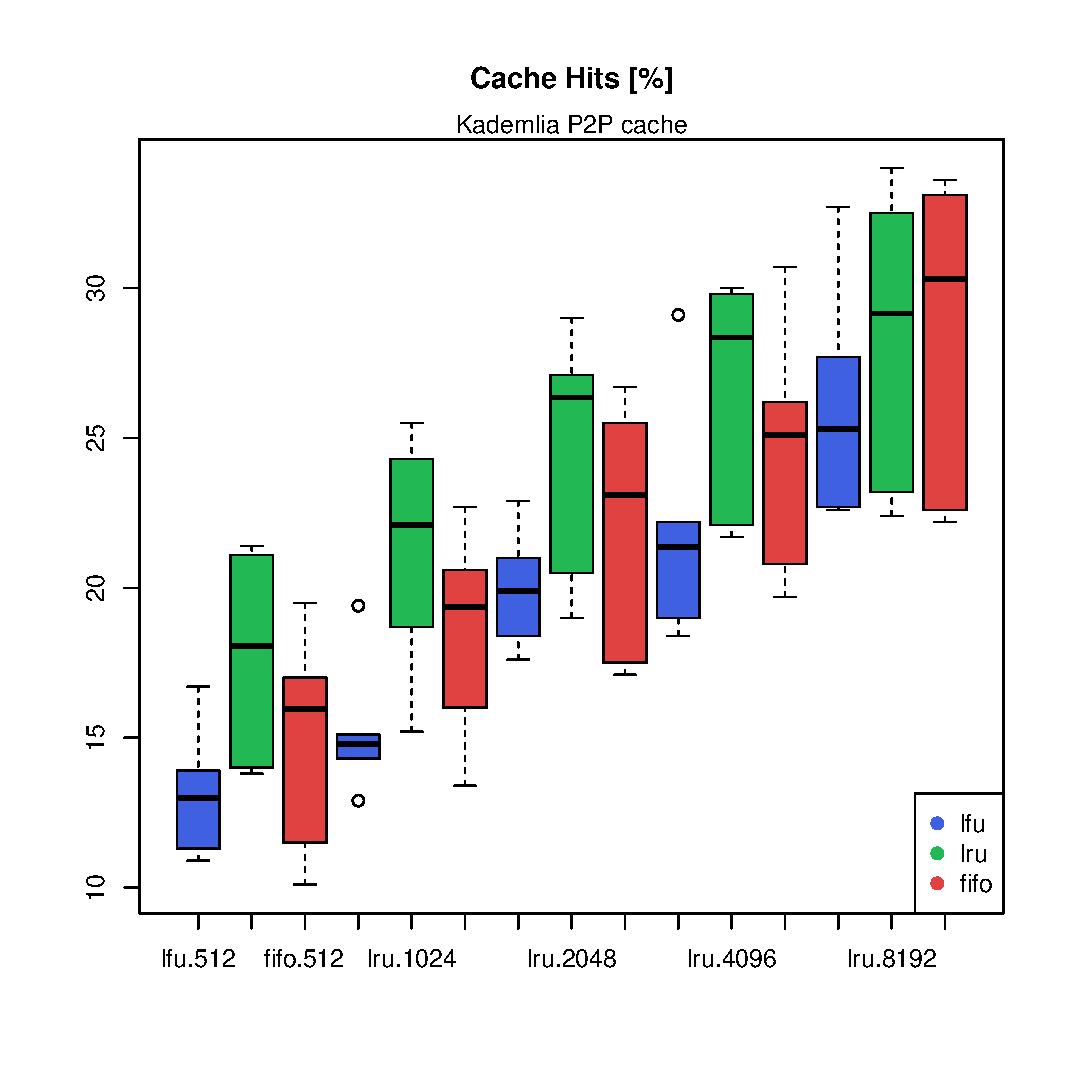
\includegraphics[width=0.7\linewidth]{img/tests/p2p_combined_all.eps}
\end{figure}
\end{frame}

\begin{frame}
\frametitle{Wyniki eksperymentów - Wnioski}

TOOD: !!!!
\end{frame}


\begin{frame}[allowframebreaks]
\frametitle{Literatura}
\bibliographystyle{plainnat}
\bibliography{document.bib}
\end{frame}


\end{document}
